%% LyX 2.0.6 created this file.  For more info, see http://www.lyx.org/.
%% Do not edit unless you really know what you are doing.
\documentclass[11pt,twoside,english,italian]{report}
\renewcommand{\ttdefault}{mathpazo}
\usepackage[T1]{fontenc}
\usepackage[utf8]{inputenc}
\usepackage[a4paper]{geometry}
\geometry{verbose}
\setcounter{secnumdepth}{3}
\setcounter{tocdepth}{3}
\usepackage{fancybox}
\usepackage{calc}
\usepackage{amsmath}
\usepackage{amssymb}
\PassOptionsToPackage{normalem}{ulem}
\usepackage{ulem}

\makeatletter

%%%%%%%%%%%%%%%%%%%%%%%%%%%%%% LyX specific LaTeX commands.
%% Because html converters don't know tabularnewline
\providecommand{\tabularnewline}{\\}

%%%%%%%%%%%%%%%%%%%%%%%%%%%%%% User specified LaTeX commands.

\newlength\tindent
\setlength{\tindent}{\parindent}
\setlength{\parindent}{0pt}
\renewcommand{\indent}{\hspace*{\tindent}}

\providecommand{\coursename}{Logica e Algebra 2}
\providecommand{\documentsubtitle}{Appunti}
\providecommand{\annoacc}{2011-2012}
\providecommand{\principaladviser}{Prof. Alessandra Cherubini}
\providecommand{\firstauthor}{Edoardo Pasi}
\providecommand{\firstauthorid}{edogay}
\providecommand{\secondauthor}{Davide Tateo}
\providecommand{\secondauthorid}{799311}
\title{Logica e Algebra 2}
\author{\firstauthor, \secondauthor}

 
\usepackage{tikz}

\usepackage{color}   %May be necessary if you want to color links
\usepackage{hyperref}
\hypersetup{
    colorlinks=true, %set true if you want colored links
    linktoc=all,     %set to all if you want both sections and subsections linked
    linkcolor=black,  %choose some color if you want links to stand out
}

\usepackage{booktabs}
\usepackage{listings}
\lstset{columns=fullflexible}

\usepackage{wasysym}

\usepackage{amsthm}
\newtheoremstyle{note} % name
{\topsep} 	% Space above
{\topsep} 	% Space below
{\small}		% Body font
{}		% Indent amount
{\small\bfseries}% Theorem head font
{:}		% Punctuation after theorem head
{.5em}	% Space after theorem head
{}		% Theorem head spec (can be left empty, meaning ‘normal’)

\usepackage{fancyhdr}%% Cambia il carattere delle didascalie delle figure %%
\usepackage[font=small,format=plain,labelfont=bf,up,textfont=it,up]{caption}

\usepackage{comment}

%per le tabelle lunghe e particolari
\usepackage{lscape}
%include il comando per creare la pagina dei titoli
\usepackage{settings/frontesp}

\makeatother

\usepackage{babel}
\begin{document}
\titlep

\tableofcontents{}

\selectlanguage{english}%
\global\long\def\veraw#1#2#3{#1\models_{#2}#3}


\global\long\def\vera#1#2{#1\models#2}


\global\long\def\nonvera#1#2{#1\nvDash#2}


\global\long\def\nonveraw#1#2#3{#1\nvDash_{#2}#3}


\global\long\def\nonSem#1#2{#1\nvdash#2}


\global\long\def\nonTeor#1#2{\nvdash_{#1}#2}


\global\long\def\nonSemW#1#2#3{#1\nvdash_{#2}#3}


\global\long\def\verita#1#2{#1\in V(#2)}


\global\long\def\entail#1#2{#1\models#2}


\global\long\def\semantica#1#2#3{#1\vdash_{#2}#3}


\global\long\def\teolm#1#2{\vdash_{#1}#2}


\global\long\def\semGen#1#2{#1\vdash#2}


\global\long\def\boxx#1{\square#1}


\global\long\def\diam#1{\diamond#1}


\global\long\def\dia{\diamond a}


\global\long\def\boa{\boxx a}


\global\long\def\noa{\neg a}


\global\long\def\forhten#1#2#3{\forall#1#2\implies#3}


\global\long\def\implica#1#2{#1\implies#2}


\global\long\def\teorema#1{\vdash_{\Lambda}#1}


\global\long\def\teorGamma#1{\Gamma\vdash_{\Lambda}#1}


\global\long\def\teoa{\teorGamma a}


\global\long\def\teoremaDi#1{\vdash_{#1}}


\global\long\def\consist{\mbox{\ensuremath{\Lambda}}-consistente}


\global\long\def\consMax{\Lambda-consistente\: massimale}


\global\long\def\veraCanAlfa#1{\vera{M^{\Lambda}}{_{\alpha}}#1}


\global\long\def\veraCA{\vera{M^{\Lambda}}{_{\alpha}}a}


\global\long\def\veraCan#1#2{\vera{M^{\Lambda}}{_{#1}}#2}


\global\long\def\nonveraCan#1#2{\nonveraw{M^{\Lambda}}{#1}{#2}}


\global\long\def\consMaxLog#1{#1-consistente\ massimale}


\global\long\def\relazCAB#1#2{\{a\ |\ \boa\in#1\}\subseteq#2}


\global\long\def\relazCAD#1#2{\{\diamond b\ |\ b\in#2\}\subseteq#1}


\global\long\def\andoria#1{a_{1}\wedge...\wedge a#1}


\global\long\def\andbox#1{\boa_{1}\wedge\dots\wedge\boxx a#1}


\global\long\def\neci#1#2{[#1]#2}


\global\long\def\posi#1#2{<#1>#2}


\global\long\def\necf#1{[F]#1}


\global\long\def\posf#1{<F>#1}


\global\long\def\necp#1{[P]#1}


\global\long\def\posp#1{<P>#1}


\global\long\def\verins#1{\Vert#1\Vert^{\mu}}


\global\long\def\verinsx#1#2{\Vert#1\Vert^{\mu^{#2}}}


\global\long\def\cardinal#1{\Vert#1\Vert}


\global\long\def\alue{AL\mbox{\ensuremath{\mathcal{UE}}}}


\global\long\def\alc{AL\mbox{\ensuremath{\mathcal{\mathcal{C}}}}}
	

\global\long\def\globally#1{\mathcal{G}#1}


\global\long\def\eventually#1{\mathcal{F}#1}


\global\long\def\next#1{\mathcal{X}#1}


\global\long\def\until#1#2{#1\mathcal{U}#2}


\global\long\def\release#1#2{#1\mathcal{R}#2}
\selectlanguage{italian}%




\chapter{Introduzione}

\label{cap:introduction}


\section{Intro}

Se voi signorine finirete questo corso, e se sopravviverete sarete
dispensatori di fbf e pregherete per modellizzare sistemi assurdi
in modo ancora più assurdo, ma fino a quel giorno non siete altro
che buoni annulla convinti che tutti i cretesi sono stupidi e forse
mentono.

Lasciate il formaggio fuori dall'aula.


\global\long\def\veraw#1#2#3{#1\models_{#2}#3}
 

\global\long\def\vera#1#2{#1\models#2}


\global\long\def\verita#1#2{#1\in V(#2)}
 

\global\long\def\entail#1#2{#1\models#2}
 

\global\long\def\semantica#1#2#3{#1\vdash_{#2}#3}


\global\long\def\semGen#1#2{#1\vdash#2}


\global\long\def\boxx#1{\square#1}


\global\long\def\diam#1{\diamond#1}


\global\long\def\dia{\diamond a}


\global\long\def\boa{\boxx a}


\global\long\def\forhten#1#2#3{\forall#1#2\Rightarrow#3}


\global\long\def\implica#1#2{#1\Rightarrow#2}



\chapter{Introduction}

$a$ è vera nel mondo $\alpha$, e scriviamo $\mu\models_{\alpha}a$

se
\begin{itemize}
\item $a$ è una lettera enunciativa allora deve valere $\verita a{\alpha}$ 
\item $a$ è del tipo: $a\lor b$ .... allora.... $\mu\models_{\alpha}a$
oppure $\mu\models_{\alpha}b$
\end{itemize}

\section{Formule di Logica modale e significato}

\begin{tabular}{|c|c|c|}
\hline 
$\diam{}{a\Rightarrow}\boxx a$  & funzione parziale & $\forhten{\alpha}{:\,\alpha R\beta,\:\beta R\gamma}{\beta}=\gamma$\tabularnewline
\hline 
\end{tabular}

Funzione parziale, dimostrazione

.

Ip) funzione parziale 

Ts) $\diam{}{a\Rightarrow}\boxx a$

.

$\diam{}a$ falsa allora dato che l'antecedente è falso di ha $\implica{\diam{}a}{\boxx a}$

$\diam{}a$ vera allora $\exists\beta$:$\alpha R\beta$ e$\in V(\beta)$,
ma dato che la funzione è parziale questo $\beta$ è unico !

da cui $\vera{\mu}{\implica{\diamond a}{\boxx a}}$

.

.

Ip) $\diam{}{a\Rightarrow}\boxx a$

Ts) funzione parziale

.

.

Per assurdo: suppongo non che la funzione non sia parziale. Se è così
$\exists\alpha:$ $\alpha R\beta,$ $\alpha R\gamma$, considero un
modello in cui V(A) = \{$\beta$ \} , $\boxx A$ non vale in $\alpha$
dato che A è falsa in $\gamma$, il che contraddice l'ipotesi (BAM!)\\\\

\begin{tabular}{|c|c|c|}
\hline 
$\diam{}{a\iff}\boxx a$  & funzione totale & $\forall\alpha\exists\,!\,\beta:\:\alpha R\beta$ \tabularnewline
\hline 
\end{tabular}\\\\

non ci sono ``conti'' da fare, R è seriale sse R è seriale $\boxx a\implies\diam a$
, e se R è una funzione parziale $\implica{\diam a}{\boxx a}$

quindi dato che l'implica prevede un and di implica da una parte e
dall'altra per definizione abbiamo la tesi

.

.

\begin{tabular}{|c|c|c|}
\hline 
$\diam{}{a\Rightarrow}\boxx{\diam a}$  & relazione euclidea & $\forhten{\alpha,\beta,\gamma}{:\:(\alpha R\beta,\:\alpha R\gamma)}{\beta}R\gamma$
da cui anche: $\beta$R$\beta$, $\gamma R\gamma$, $\gamma$R$\beta$\tabularnewline
\hline 
\end{tabular} \\\\

Ip) relazione euclidea

Ts) $\diam{}{a\Rightarrow}\boxx{\diam a}$ 

Suppongo sia vero l'antecedente (se falso ho finito), quindi vale:
$\dia$ da cui: $\vera{\mu}{\dia}$

dato che $\dia$ si ha che esiste almeno un $\beta$ tale che in beta
vale a 

solo un beta: autoanello perché euclidea e quindi $\boxx{\dia}$

diversi beta: ognuno dei vari $\beta'$, $\beta''$ , ecc. sono in
relazione con $\beta$, dato che la relazione è euclidea, pertanto
dato che in $\beta$ vale $a$, in ognuno di loro vale $\dia$ \\

Ip)$\diam{}{a\Rightarrow}\boxx{\diam a}$ 

Ts) relazione euclidea

Per assurdo, suppondo valga ip) ma non la tesi

Considero un Frame in cui: $\alpha R\beta,$ $\alpha R\gamma,$ $\beta R\gamma$
ma NON $\beta R\gamma$ cioè si ha un frammento in cui non vale l'euclidea.
Poniamo che il modello sia tale che $V(A)$$=\{\gamma\}$

In queste ipotesi vale $\dia$ dato che in $\gamma$ vale $a$. In
$\beta$ non vale $a$ e neppure $\dia$ perché non ha ``uscite'',
da cui in $a$ non vale $\boxx{\dia}$ contraddicendo così l'ipotesi
(BAM!) \\\\


\section{Semantica}

$\semGen ab$ cioè a è conseguenza semantica di b, se in ogni Frame,
Modello e Mondo in cui $\vera{\mu}b$ si ha anche $\vera{\mu}a$\\

$\dia\equiv\sim\boxx{\sim a}$

Vale da sinistra a destra,

Infatti:

se $\veraw{\mu}{\alpha}{\dia}$ allora 

$\exists\beta:$$\alpha R\beta$ e $\veraw{\mu}{\beta}a$ da cui:

$\mu\nvDash_{\beta}\sim a$

per questo in $\alpha$ non vale $\boxx{\sim a}$ (perché non vale
$\sim a$ in $\beta$)

allora in $\alpha$ vale $\sim\boxx{\sim a}$ cioè $\veraw{\mu}{\alpha}{\sim\boxx{\sim a}}$
cioè la tesi. \\

Vale anche da destra a sinistra, dimostrazione simile.



\chapter{Semantica}


\section{Simboli secessari}

$\semGen ab$ cioè a è conseguenza semantica di b, se in ogni Frame,
Modello e Mondo in cui $\vera\mu b$ si ha anche $\vera\mu a$\\


$\dia\equiv\neg\boxx{\neg a}$

Vale da sinistra a destra,

Infatti:

se $\veraw\mu\alpha\dia$ allora

$\exists\beta:$$\alpha R\beta$ e $\veraw\mu\beta a$ da cui:

$\mu\nvDash_{\beta}\neg a$

per questo in $\alpha$ non vale $\boxx{\neg a}$ (perché non vale
$\neg a$ in $\beta$)

allora in $\alpha$ vale $\neg\boxx{\neg a}$ cioè $\veraw\mu\alpha{\neg\boxx{\neg a}}$
cioè la tesi. \\


Vale anche da destra a sinistra, dimostrazione simile. \\



\section{Logiche}

Una logica $\Lambda$ su L è un insieme di fbf su L che: 
\begin{itemize}
\item contiene tutte le tautologie 
\item è chiusa rispetto al Modus Ponens 
\end{itemize}
Ad esempio; $PL(\phi)$ cioè i teoremi della logica proposizionale

Altro esempio $\Lambda_{C}=\{a\,|\,\vera F{a\: per}\ ogni\ F\in C\}$

infatti: 
\begin{itemize}
\item contiene tutte le tautologie perché sono vere mondo per mondo dappertutto 
\item MP : suppongo che in un mondo $\alpha$ accada che: $\nonveraw{\mu}{\alpha}b$
, $\veraw{\mu}{\alpha}a$ . Se vale anche $\veraw{\mu}{\alpha}{\implica ab}$
... l'antecedente è vero, quindi dato che l'implicazione è vera, deve
essere vero anche il conseguente da cui non può che essere $\veraw{\mu}{\alpha}b$ 
\end{itemize}
Una logica si dice \textbf{uniforme }se è chiusa rispetto a sostituzioni
uniformi cioè se sostituendo a una lettere uguali formule uguali in
una tautologia, ottengo una tautologia.

Es. $\Lambda_{C}=\{a\,|\,\vera F{a\: per}\ ogni\ F\in C\}$ NON è
uniforme infatti se considero $V(A)=S$, dove S sono tutti gli stati
possibili (mondi), vale anche $\veraw{\mu}{\alpha}A$, e cioè A è
una tautologia, se al posto di A sostituisco $B\wedge\neg B$ (falsa
in ogni modello e mondo) non ottengo una tautologia.\\
 \\


\textbf{\emph{\large{{{{Teorema}}}}}}{\large \par}

Sono equivalenti: 
\begin{enumerate}
\item $\Lambda$ è normale 
\item per ogni intero n $\geq0$,


$\teorema{a1\wedge a2\wedge...\wedge an}\implies a$ implica $\teorema{\boa1\wedge\boa2\wedge...\wedge\boa n}\implies\boa$

\item valgono:

\begin{enumerate}
\item $\teorema{\boxx T}$ 
\item $\teorema{\boa\wedge\boxx b}\implies\boxx{(a\wedge b)}$ 
\item $\teorema{\implica ab}$ implica $\teorema{\boa\implies\boxx b}$ 
\end{enumerate}
\end{enumerate}
Dimostrazione

$1\implies$2

per induzione.

se n = 0 allora $\teorema a$ allora $\teorema{\boa}$ per la regola
RN che vale in $\Lambda$ per ipotesi

se n > 0 (passo induttivo) suppongo valga l'antecedente, altrimenti
2 vale senz'altro;

Ricordiamo che $a1\wedge a2\wedge...\wedge an\implies a\equiv a1\wedge a2\wedge...a_{n-1}\implies(an\implies a)$ 


\begin{savequote}[60mm]
Senza dubbio questo era un piano eccellente, semplice e davvero ben congegnato. \\
C'era solo una difficoltà: che Alice non aveva la più piccola idea di come realizzarlo.
\qauthor{Lewis Carroll} \end{savequote}


\chapter{Verso la decidibilità - Logica determinata}


\section{Insieme $\Lambda$ consistente e sue proprietà}

Sia $\Lambda$ una logica (cioè ha tutte le tautologie ed è chiusa
rispetto al Modus Ponens)	

$\Gamma$ si dice $\Lambda$-consistente se: $\nonSinW{\Gamma}{\Lambda}{\bot}$,
dove $\bot=A\wedge\neg A$

$\Delta$ si dice $\Lambda$-consistente massimale se per ogni fbf
$a$ $a\in\Delta$ oppure $\neg a\in\Delta$ $ $\\


\textbf{Proprietà:} $ $ 
\begin{enumerate}
\item Se $\teoa$ e $\Gamma\subseteq\Delta$ allora $\Delta\teorema a$.
Ovvero se alcune premesse non mi servono posso comunque metterle per
dedurre una formula 
\item Se $\teorGamma a$ e $\Lambda\subseteq\Lambda'$ allora $\Gamma\vdash_{\Lambda'}a$.
Ovvero quello che posso dedurre in una logica più scarna (es. PL)
lo posso dedurre anche in una più ricca che la contiene (es. Modale) 
\item se $a\in\Gamma$ allora $\teoa$ . \\
 Infatti $\teorema{a\implies a}$ è un teorema dato che $a\implies a$
è una tautologia 
\item $\{a|\teoa\}$ è la minima logica che contiene $\Gamma\cup\Lambda$.
Infatti posso dedurre tutte le tautologie da $\Gamma$, anche se non
userò nessuna formula di $\Gamma$ ma solo quelle che già sono nella
logica $\Lambda$ $ $ 
\item Se $\teoa$ e $\{a\}$$\teorema b$ allora $\teorGamma b$ \\
 Infatti: per dedurre $a$ uso regole di inferenza, formule di $\Gamma$,
assiomi di $\Lambda$. Per arrivare in $b$ uso assiomi di $\Lambda$
e regole di inferenza, quindi posso arrivare da $\Gamma$ direttamente
in $b$ usando formule di $\Gamma$, regole di inf. e assiomi di $\Lambda$ 
\item Se $\teoa$ e $\teorGamma{\implica ab}$ allora $\teorGamma b$, dato
che $\Lambda$ è chiusa rispetto al MP 
\item $\Gamma\cup\{a\}\teorema b$ se e solo se $\teorGamma{\implica ab}$
\\
 \textbf{Andata}: $\teorema{a_{1}\wedge...\wedge a\wedge...\wedge}a_{n}\implies b$
(per definizione di teorema), si può portare $a$ alla destra dell'implicazione
$\teorema{a_{1}\wedge...\wedge}a_{n}\implies(a\implies b)$ \\
 \textbf{Ritorno}: $\teorema{a_{1}\wedge}...\wedge a_{n}\implies(a\implies b)$,
basta portare $a$ tra le $ $and. 
\item $\teoa$ se e solo se $\Gamma\cup\{\neg a\}$ non è $\Lambda$-consistente
\\
 \\
 \textbf{Andata}: $\teoa$, $\Gamma\teorema{\neg a}$, posso dedurre
$\bot$ che è contro la definizione di $\Lambda$-consistenza\\
 \textbf{Ritorno}: Se$ $$\Gamma\cup\{\neg a\}$ non è $\Lambda$-consistente,
allora $\Gamma\cup\{\neg a\}\teorema{\bot}$ da cui per 7. \\
 $\Gamma\teorema{\neg a\implies\bot}$ (sposto $\neg a$ a destra
e metto l'implica), \\
 Dato che $(\neg a\implies\bot)\implies a$ è una tautologia, per
MP ottengo\\
 $a$ 
\item $\Gamma$ è $ $$\consist$ se e solo se $\exists\beta:\nonSem{\Gamma}{_{\Lambda}\beta}$
\\
 \textbf{Andata}: Basta prendere $\neg a\wedge a$\\
 \textbf{Ritorno}: Se deducessi tutte le formule ($\neg$$\exists\beta:\nonSem{\Gamma}{_{\Lambda}\beta}$
significa $\forall\beta:\teorGamma{\beta}$) , potrei dedurre anche
$\bot$, da cui la non consistenza 
\item $\Gamma$ è $\consist$ se per ogni $a$ \\
 $\Gamma\cup\{a\}$ o $\Gamma\cup\{\neg a\}$ è $\consist$\\
 se $\teoa$ allora $ $$\Gamma\cup\{\neg a\}$ non è consistente
perché con $a$ e $\neg a$ posso dedurre $\bot$, ma $\Gamma\cup\{a\}$
lo è \\
 se $\Gamma\teorema{\neg a}$ allora $ $$\Gamma\cup\{\neg a\}$ è
consistente ma non $\Gamma\cup\{a\}$ 
\item $\bot$$\notin\Gamma$ se $\Gamma$ è $\consist$ (altrimenti potrei
dedurlo per il 3.) 
\item Se $\Delta$è $\consist\: massimale$ e $\Delta\teorema a$ allora
$a\in\Delta$\\
 se $a\notin\Delta$ allora $\neg a\in\Delta$ (dato che $\Delta$è
massimale) \\
 ma se $\Delta$ contiene $\neg a$ allora per il 2.)\\
 $\Delta\teorema{\neg a}$ , che insieme a $\Delta\teorema a$ mi
da $\Delta\teorema{\bot}$ 
\item Se $\Delta$ è $\consMax$ e $ $$a\in\Delta$. $\implica ab\in\Delta$
allora $b\in\Delta$. \\
 Lo si vede subito usando 2.) se tutti e tre, e poi 6.) (deduco $a$,
$\implica ab$, allora deduco anche $b$) 
\end{enumerate}

\section{Insieme $\Lambda$ consistente massimale}


\subsection{Lemma di Lindenbaum}

Una logica consistente ammette sempre un insieme $\Lambda$- consistente
massimale. Infatti il lemma di Lindenbaum afferma:

$(\Gamma\,\Lambda-consistente)\implies\,\exists\Delta\supseteq\Gamma\,\wedge\,(\Delta\,\Lambda-consistente\, massimale)$

Ip) $\Gamma\,\grave{e}\,\Lambda-consistente$

Ts) $\exists\Delta\supseteq\Gamma$ e $\Delta\,\grave{e}\,\Lambda-consistente\, massimale$\\


Considero tutte le formule b1, b2, b3 della logica $\Lambda$ (posso
farlo perché sono una infinità numerabile)

Chiamo $\Gamma_{0}$ un insieme che contiene una sola formula (ad
esempio una tautologia)

Dopodiché iterativamente, per ogni formula mi chiedo\\


$\Gamma_{0}$$\teorema{b1}$ ? $\begin{cases}
si: & \Gamma_{1}=\Gamma_{0}\cup b1\\
no: & \Gamma_{1}=\Gamma_{0}\cup\neg b1
\end{cases}$\\


$\Gamma_{1}$$\teorema{b2}$ ? $\begin{cases}
si: & \Gamma_{2}=\Gamma_{1}\cup b2\\
no: & \Gamma_{2}=\Gamma_{1}\cup\neg b2
\end{cases}$ 
\begin{description}
\item [{$\Delta=\underset{n\geq0}{\bigcup}\Gamma$}] (nota, questa unione
è infinita) 
\item [{$\Delta$}] è consistente massimale infatti:\end{description}
\begin{enumerate}
\item Massimale in quanto contiene $a$ oppure $\neg a$ per costruzione 
\item Consistente. Per assurdo se non lo fosse avrei: $\Delta\teorema{\bot}$\\
 cioè esiste un numero finito di formule di $\Delta$ da cui deduco
il falso,\\
 dato che è un numero finito di formule, sta in $\Gamma_{i}$ , cioè
esiste un $\Gamma_{i}$ non consistente, assurdo perché lo sono tutti
per costruzione \lightning 
\end{enumerate}
\emph{\large{{Nota:}}}{\large \par}

 
\begin{itemize}
\item Non sappiamo costruire $\Delta$ perché nasce da unione infinita 
\item Non è unico, infatti se considero formule in ordine diverse potrei
``dire'' si o no in modo diverso \\
 es. $a,\ \implica ab,\ b$ (allora $\Delta$ contiene $b$)\\
 es. $b,\ c$ (allora $\Delta$ contiene $\neg b$) 
\end{itemize}

\subsection{Teorema}

$\teoa$ se e solo se $a\in$ a tutti i quei $\Delta$ $\Lambda-consistenti\ massimali$
tali che: $\Gamma\subseteq\Delta$\\


\textbf{Andata:}

$\teoa$, anche $\Delta\teorema a$ per la 1.)

\textbf{Ritorno:}

Per assurdo, se $\nonSem{\Gamma}{_{\Lambda}a}$ allora $\Gamma\cup\{\neg a\}$
è $\consist$ (per la 8.)

da cui per Lindellman esiste $\Delta'$ che contiene $\Gamma\cup\{\neg a\}$
consistente massimale

data la consistenza $\Delta'$ non contiene $a$, il che è contro
l'ipotesi \lightning


\section{Lemma di Verità}

Sia $M^{\Lambda}(S^{\Lambda},R^{\Lambda},V^{\Lambda})$ il modello
canonico di $\Lambda$

$M^{\Lambda}\veraCanAlfa{_{\alpha}a}$ se e solo se $a\in\alpha$\\


Ip) $M^{\Lambda}\veraCanAlfa{_{\alpha}a}$

TS) $a\in\alpha$\\


Dimostrazione per \textbf{induzione} sul numero n dei connettivi della
formula $a$

\ovalbox{n=0} cioè $a$ è del tipo $A$ (lettera enunciativa) da
cui $M^{\Lambda}\veraCanAlfa{_{\alpha}a}$ se e solo se $\alpha\in V^{\Lambda}(A)$
se e solo se $A\in\alpha$

\ovalbox{Ipotesi di Induzione} $a$ con n connettivi, può essere
dei seguenti tipi: 
\begin{enumerate}
\item $\neg b$ 
\item $\implica bc$ 
\item $\boxx b$ 
\end{enumerate}
\textbf{Caso 1:} $M^{\Lambda}\veraCanAlfa{_{\alpha}a}$ se e solo
se $M^{\Lambda}\veraCanAlfa{_{\alpha}\neg b}$ se e solo se $\nonveraCan{\alpha}b$\\


$b$ ha $n-1$ connettivi (dato che $b$) ne ha $n$, quindi vale
l'ipotesi di induzione da cui:

$b\notin\alpha$, d'altra parte $\alpha$ è $\consMax$ (per come
è definito $S^{\Lambda}$) da cui:

\textbf{$b\notin\alpha$ }se e solo se \textbf{$ $}$\neg b\in\alpha$
cioè se:

$a\in\alpha$

\textbf{Caso} 2:$ $ $M^{\Lambda}\veraCanAlfa{_{\alpha}a}$ se e solo
se

Caso 21: $\nonveraCan{\alpha}b$

Caso 22: $\veraCan{\alpha}c$\\


\textbf{Caso 21}: $\nonveraCan{\alpha}b$ \\


Il numero di connettivi di $b$ e di $c$ sommati dà $n-1$

quindi per ipotesi induttiva $\nonveraCan{\alpha}b$ se e solo se
$b\notin\alpha$

se e solo se $\neg b\in\alpha$ (per la compattezza max di $\Lambda$)
\textbf{({*})}

D'altra parte $\neg b\implies(b\implies c)$ è una tautologia della
PL e quindi è un teorema di $\Lambda$ (perché un logica contiene
tutte le tautologie)

e quindi $\neg b\implies(b\implies c)$ $\in\alpha$ \textbf{({*}{*})}

da cui per MP con \textbf{({*})} e \textbf{({*}{*})} si ha che $b\implies c$
appartiene ad $\alpha$\\
 \\
 \textbf{Caso 22}: $M^{\Lambda}\veraCanAlfa{_{\alpha}c}$\\


Vale l'ipotesi di induzione da cui:

quindi per ipotesi induttiva $\veraCan{\alpha}c$ se e solo se $c\in\alpha$
\textbf{({*})}

D'altra parte $c\implies(b\implies c)$ è una tautologia della PL
e quindi è un teorema di $\Lambda$ (perché un logica contiene tutte
le tautologie)

e quindi $c\implies(b\implies c)$ $\in\alpha$ \textbf{({*}{*})}

MP \textbf{({*}) }e \textbf{({*}{*}) }ci dà $b\implies c$ appartiene
ad $\alpha$\\
 \\
 \textbf{Caso 3}: $a$ è del tipo $\boxx b$\\


Ip)$M^{\Lambda}\veraCanAlfa{_{\alpha}\boxx b}$

Ts)$\boxx b\in\alpha$\\


Dall'ipotesi segue che $\forall\beta:(\alpha,\beta)\in R^{\Lambda}$
si ha: $M^{\Lambda}\veraCanAlfa{_{\beta}b}$ (questo per la definizione
di $\boxx x$)

$b$ ha $n-1$ connettivi quindi vale per lei l'ipotesi di induzione:

$b\in\beta$

\ovalbox{\parbox[t][1\totalheight][c]{0.9\textwidth}{%
$(\alpha,\beta)\in R^{\Lambda}$ se e solo se: $\{a\ |\ \boa\in\alpha\}\subseteq\beta$

$\alpha\in V^{\Lambda}(A)$ se e solo se: $A\in\alpha$%
}} \\


Ognuno dei $\beta$ con cui $\alpha$ è in relazione è $\consMax$
(per come sono definiti gli stati del modello canonico) e ognuno contiene
l'insieme $\{a\ |\ \boa\in\alpha\}$ (per come è definita la relazione
$R^{\Lambda}$)

$\Gamma\teorema a$ se e solo se $a$ appartiene a tutti i $\Delta_{i}$
$\consMax$ con $\Gamma\subseteq\Delta_{i}$

$\beta\teorema b$ se e solo se $b$ appartiene a tutti i $\Delta_{i}$
$\consMax$ con $\beta\subseteq\Delta_{i}$

$\{a\ |\ \boa\in\alpha\}$ è consistente massimale ed è contenuto
in $\beta$ e quindi

$b\in\{a\ |\ \boa\in\alpha\}$ da cui per la proprietà 3. di insieme
consistente si ha anche

$\{a\ |\ \boa\in\alpha\}$ $\teorema b$, inoltre, per la 2. definizione
equivalente di Logica Normale ``aggiungo $\square$ ad entrambi i
lati'' da cui:

$\{\boa\ |\ \boa\in\alpha\}$ $\teorema{\boxx b}$, dato che $\{\boa\ |\ \boa\in\alpha\}$
è consistente massimale. per la 12. delle proprietà di consistenza
si ha anche

$\boxx b\in\{a\ |\ \boa\in\alpha\}$ da cui, a maggior ragione $\boxx b\in\alpha$\\


Ip) $\boxx b\in\alpha$

TS) $M^{\Lambda}\veraCanAlfa{_{\alpha}\boxx b}$\\
\\
 Se $\boxx b\in\alpha$ per definizione di $R^{\Lambda}$ per ogni
mondo $\beta$ con $(\alpha,\beta)\in R^{\Lambda}$ si ha $b\in\beta$

Notiamo che $b$ ha $n-1$ connettivi, quindi vale l'ipotesi di induzione
e quindi:

$ $$b\in\beta$ se e solo se $M^{\Lambda}\veraCanAlfa{_{\beta}b}$

Dato che questo vale $ $per ogni $\beta$ in relazione con $\alpha$,
si ha: $M^{\Lambda}\veraCanAlfa{\beta\boxx b}$


\section{Correttezza e completezza della logica K rispetto a tutti i Frame}

Dimostriamo che la logica K (minima logica modale normale) è corretta
e completa

Ip) $\teolm Ka$

Ts)$\vera Fa$\\


A1, A2, A3 sono tautologie e quindi valide su tutti i frame

MP, sia la regola di necessitazione (RN) fanno passare da formule
valide su un frame a formule valide su quello stesso frame.

Essendo $a$ l’ultima formula di una sequenza finita di fbf che o
sono istanze degli assiomi A1, A2, A3, K o sono ottenute da fbf precedenti
tramite MP o RN, è una fbf valida su ogni frame.\\
 \\
 Ip) $\vera Fa$

Ts)$\teolm Ka$ \\
 \\
 Supponiamo $\nonTeor Ka$, allora per il corollario del lemma di
verità\\


\ovalbox{\parbox[t][1\totalheight][c]{0.9\textwidth}{%
Per ogni formula $a$, sia $\Lambda$ una logica, si ha $\vera{M^{\Lambda}}a$
se e solo se $\teorema a$, dove $M^{\Lambda}$ è il modello canonico%
}} \\


Si avrebbe: $\nonvera{M^{K}}a$ da cui anche

$\nonvera{F^{K}}a$, cioè $a$ non valida sul frame su cui $M^{K}$
è costruito quindi:

$\nonvera Fa$ (infatti esiste almeno un frame, $F^{K},$ in cui non
è valida $a$) il che però è contro l'ipotesi \lightning.


\section{Correttezza e completezza della logica K4 rispetto ai Frame transitivi}

Nota: K4 è costruita a partire dalla logica K a cui si aggiunge l'assioma
della transitività $\boa\implies\boxx{\boa}$ \\
 Ip)$\teolm{K4}a$

Ts) $\entail Fa$ con F frame transitivo\\
 \\
 Simile al caso precedente in cui anche 4 è valido in quando il frame
è transitivo\\


Ip) $\entail Fa$ con F frame transitivo (cioè la cui relazione è
transitiva)

Ts)$\teolm{K4}a$\\
 \\
 Per procedere con una dimostrazione sulla falsa riga della precedente
abbiamo bisogno di dimostrare la transitività di $R^{K4}$

cioè della relazione $R^{K4}$ del modello canonico $M^{K4}=(S^{K4},R^{K4},V^{K4})$,
servirà ragionando per assurdo.\\


\textbf{Transitività di $R^{K4}$ }

se $(\alpha,\beta)\in R^{K4}$, $(\beta,\gamma)\in R^{K4}$ allora
$(\alpha,\gamma)\in R^{K4}$

cioè deve avvenire che: $\{a\ |\ \boa\in\alpha\}\subseteq\gamma$
(definizione di essere in relazione $\alpha R^{K4}\gamma$ del modello
canonico)

se $\boa\in\alpha$ , ricordando che:

$\alpha$ è un insieme $K4-consistente\ massimale$,

4 è un teorema della logica

i teoremi di una logica appartengono a tutti gli insiemi consistenti
massimali rispetto a quella logica quindi

$\alpha$, così come ogni insieme $K4-consistente\ massimale$, contiene
anche $\boa\implies\boxx{\boa}$ (4) da cui

\selectlanguage{english}%
$\boxx{\boa}\in\alpha$\foreignlanguage{italian}{.}

\selectlanguage{italian}%
$\{a\ |\ \boa\in$$\alpha\}\subseteq\beta$ (per ipotesi $\alpha R^{K4}\beta$)

ma per ogni formula $\boa\in\alpha$ si ha che $\boxx{\boxx a}\in\alpha$
e quindi: $\{\boa\ |\ \boxx{\boxx a}\in\alpha\}\subseteq\beta$ da
cui $\{\boa\ |\ \boxx a\in\alpha\}\subseteq\beta$

\selectlanguage{english}%
$\{a\ |\ \boa\in$$\beta\}\subseteq\gamma$\foreignlanguage{italian}{
(per ipotesi $\beta R^{K4}\gamma$), ma le formule del tipo $\boa$
contenute in $\beta$ sono le stesse contenute in $\alpha$, quindi
si ha anche:}

\selectlanguage{italian}%
$\{a\ |\ \boa\in$$\alpha\}\subseteq\gamma$ cioè $(\alpha,\gamma)\in R^{K4}$
\foreignlanguage{english}{}\\
\foreignlanguage{english}{ }\\
\foreignlanguage{english}{ }A questo punto possiamo usare in modo
proficuo il corollario del lemma di verità.

Dimostriamo la tesi per assurdo: supponiamo che $\nonTeor{K4}a$

allora per il corollario del teorema di verità si avrebbe anche $\nonvera{M{}^{K4}}a$

e in particolare si avrebbe $\nonvera{F^{K4}}a$, cioè si avrebbe
un Frame transitivo (infatti $R^{K4}$ è transitiva) nel quale non
è valida $a$

ma ciò contraddice l'ipotesi $\entail Fa$ (con $F$ transitivo) \lightning\\



\section{Teorema di Raggiungibilità}

$(\alpha,\beta)\in R^{\Lambda}$ se e solo se $\relazCAB{\alpha}{\beta}$
se e solo se \foreignlanguage{english}{$\relazCAD{\alpha}{\beta}$}
\\
 Ip)$\relazCAB{\alpha}{\beta}$

Ts)$\relazCAD{\alpha}{\beta}$\\

\begin{description}
\item [{Per}] assurdo supponiamo che
\end{description}
$b\in\beta$ e che $\diamond b\notin\alpha$,

\selectlanguage{english}%
$\neg\diamond b\in\alpha$\foreignlanguage{italian}{ (dato che $\alpha$)
è $\consMax$}

\selectlanguage{italian}%
$\boxx{\neg b\in\alpha}$ (equivalenza $\boxx{\neg a}$ $\equiv$$\neg\dia$)
da cui

$\neg b\in\beta$ (definizione di $\boxx x$ e considerato $\alpha R^{\Lambda}\beta$)

il che è assurdo perché $b\in\beta$, e $\beta$ è $\consMax$\lightning\\


Ip)$\relazCAD{\alpha}{\beta}$

Ts)$\relazCAB{\alpha}{\beta}$\\
 Per assurdo supponiamo cioè che

$\boa\in\alpha$ e $a\notin\beta$

$\neg a\in\beta$ (dato che $\beta$ è $\consMax$)

$\diamond\neg a\in\alpha$ (infatti $\alpha R^{\Lambda}\beta$ e in
$\beta$ è vera $\neg a$, quindi $a$ ha almeno un successore nel
quale $\neg a$ è vera)

$\neg\boxx{a\in\alpha}$ contro l'ipotesi della consistenza e massimalità
di $\alpha$\lightning\\




\chapter{Logiche modali particolari e Decibilità (Finalmente!)}





\chapter{Decidibilità Delle Logiche Modali}


\section{Filtrazione}

Dato una logica $\Lambda$ e una formula a, si può garantire che esiste
un modello $\mu$, con un numero di mondi limitato da f(n), con n
numero di sottoformule di a tale che:

$\teoremaDi{\Lambda}a\iff\vera{\mu}a$

Dimostrazione.

Ip) $a\in\Gamma\implies sottoformule(a)\subseteq\Gamma$

Ts) $\exists\mu:\,\teoremaDi{\Lambda}a\iff\vera{\mu}a$

sia $\mu$=(S,R,V), consideriamo la seguente relazione:

$\sim_{\Gamma}\subseteq S\times S$

che gode della seguente proprietà:

$\Gamma_{\alpha}=\{a\in\Gamma\,|\,\veraw{\mu}{\alpha}a\}$

$\alpha\sim_{\Gamma}\beta\iff\Gamma_{\alpha}=\Gamma_{\beta}$

Si può notare che $\sim_{\Gamma}$ è una relazuione di equivalenza,
Infatti:
\begin{enumerate}
\item è simmetrica\\
$\alpha\sim_{\Gamma}\alpha\iff\Gamma_{\alpha}=\Gamma_{\alpha}$
\item è riflessiva\\
$\alpha\sim_{\Gamma}\beta\iff\Gamma_{\alpha}=\Gamma_{\beta}\iff\beta\sim_{\Gamma}\alpha$
\item è transitiva:\\
$\alpha\sim_{\Gamma}\beta\wedge\alpha\sim_{\Gamma}\gamma\iff\Gamma_{\alpha}=\Gamma_{\beta}=\Gamma_{\gamma}\iff\gamma\sim_{\Gamma}\beta$
\end{enumerate}
Posso allora considerare l'insieme quoziente:

$S_{\Gamma}=S/\sim_{\Gamma}$

Si può dimostrare con il teorema di fattorizzazzione delle applicazioni
che:

$|S_{\Gamma}|\leq2^{|\Gamma|}$

\begin{center} 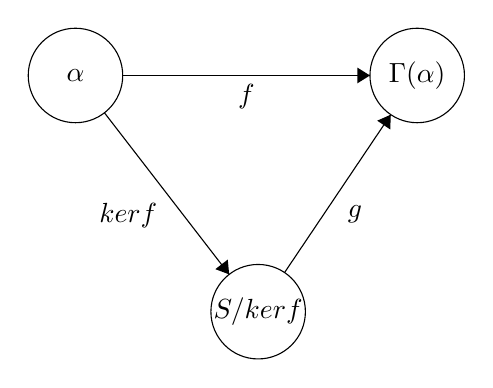
\begin{tikzpicture}[scale=0.2] \tikzstyle{every node}+=[inner sep=0pt] \draw [black] (22.1,-16.4) circle (3); \draw (22.1,-16.4) node {$\alpha$}; \draw [black] (43.8,-16.4) circle (3); \draw (43.8,-16.4) node {$\Gamma(\alpha)$}; \draw [black] (33.7,-31.4) circle (3); \draw (33.7,-31.4) node {$S/kerf$}; \draw [black] (35.38,-28.91) -- (42.12,-18.89); \fill [black] (42.12,-18.89) -- (41.26,-19.27) -- (42.09,-19.83); \draw (39.36,-25.24) node [right] {$g$}; \draw [black] (25.1,-16.4) -- (40.8,-16.4); \fill [black] (40.8,-16.4) -- (40,-15.9) -- (40,-16.9); \draw (32.95,-16.9) node [below] {$f$}; \draw [black] (23.94,-18.77) -- (31.86,-29.03); \fill [black] (31.86,-29.03) -- (31.77,-28.09) -- (30.98,-28.7); \draw (27.33,-25.31) node [left] {$kerf$}; \end{tikzpicture} \end{center}

Per dimostrarlo basta prendere:

$f:\,\alpha\rightarrow\mathcal{P}(\Gamma)$

risulta banale verificare che:

$ker\, f\equiv\sim_{\Gamma}$

e quindi, ricordando che g è iniettiva, risulta banale che:

$|S/\sim_{\Gamma}|\leq\Gamma(\alpha)$

Allora possiamo prendere il modello:

$M^{\Gamma}=(S^{\Gamma},R',V^{\Gamma})$

$R'\subseteq S^{\Gamma}\times S^{\Gamma}$

con R' che soddisfi le seguenti proprietà:

F1) $(\alpha,\,\beta)\in R\implies([\alpha],\,[\beta])\in R'$

F2) $([\alpha],[\beta])\in R'\implies\forall\boxx b\in\Gamma,\,\veraw{\mu}{\alpha}{\boxx b}\implies\veraw{\mu}{\beta}b$

Una relazione che gode delle proprietà F1 e F2 si chiama $\Gamma$-filtrazione
della relazione R.

prendiamo infine:

$V^{\Gamma}:\,\Phi\cap\Gamma\rightarrow\mathcal{P}(S^{\Gamma})$

che gode della seguente proprietà:

presa una formula atomica $A\in\Phi\cap\Gamma$

$\alpha\in V^{\Gamma}(A)\iff\alpha\in V(A)$


\subsection{Teorema}

Esiste almeno una relazione che gode delle proprietà F1 e F2:

$R^{\sigma}\subseteq S^{\Gamma}\times S^{\Gamma}$

così definita:

$([\alpha],[\beta])\in R^{\sigma}\iff\exists\delta\in[\alpha],\eta\in[\beta]\,:\,(\delta,\,\eta)\in R$

La proprietà F1 è dimostrata banalmente.

Dimostriamo F2

Ip) $([\alpha],[\beta])\in R^{\sigma}$, $\boxx{b\in\Gamma}$, $\veraw{\mu}{\alpha}{\boxx b}$

Ts) $R^{\delta}$gode della proprietà F2

supponiamo che:

$\exists\delta,\eta\,:\,\delta R\eta\wedge\delta\in[\alpha]\wedge\eta\in[\beta]$

avremo che:

$\veraw{\mu}{\delta}{\boxx b}$

$\veraw{\mu}{\eta}b$

e quindi:

$\veraw{\mu}{\beta}b$\\



\section{Lemma di Filtrazione}

dato un insieme$\Gamma$ chiuso rispetto alle sottoformule di a, con
$a\in\Gamma$

$\veraw{\mu}{\alpha}{a\iff}\veraw{\mu^{\Gamma}}{\alpha}a$

per ogni $\mu^{\Gamma}$$\Gamma$-filtrazione di $\mu$

Dimostrazione:

Ts) $\veraw{\mu}{\alpha}{a\iff}\veraw{\mu^{\Gamma}}{[\alpha]}a$

Ip) $\mu^{\Gamma}$$\Gamma$-filtrazione di $\mu$

Per induzione sul numero di connettivi di a

Caso Base, n=0:

a non ha connettivi, allora $a\equiv A$

$\veraw{\mu}{\alpha}A\iff\alpha\in V(A)\iff\alpha\in V^{\Gamma}(A)\iff\veraw{\mu^{\Gamma}}{[\alpha]}a$

Ipotesi di induzione: il teorema vale per ogni formula di $\Gamma$
con m<n connettivi.

a può essere:
\begin{enumerate}
\item $\neg b$
\item $b\implies c$
\item $\boxx b$
\end{enumerate}
Caso 1:

$\veraw{\mu}{\alpha}{\neg b}\iff\nonveraw{\mu}{\alpha}b\iff\nonveraw{\mu^{\Gamma}}{[\alpha]}b\iff\veraw{\mu^{\Gamma}}{[\alpha]}{\neg b}$

Caso 2:

$\veraw{\mu}{\alpha}{b\implies c}$ se e solo se $\nonveraw{\mu}{\alpha}b$
oppure $\veraw{\mu}{\alpha}c$

quindi si può affermare

$\nonveraw{\mu}{\alpha}b\iff\nonveraw{\mu^{\Gamma}}{[\alpha]}b$

$\veraw{\mu}{\alpha}c\iff\veraw{\mu^{\Gamma}}{[\alpha]}c$

ma vale almeno una delle due se e solo se

$\veraw{\mu^{\Gamma}}{[\alpha]}{b\implies c}$

Caso 3:

Ip) $\veraw{\mu}{\alpha}{\boxx b}$

Ts) $\veraw{\mu^{\Gamma}}{[\alpha]}{\boxx b}$

Consideriamo la reazione R' avente le proprietà F1 e F2

$\forall[\beta]\,:\,([\alpha],\,[\beta])\in R'\implies\veraw{\mu^{\Gamma}}{[\beta]}b$
-- per F2

allora si può affermare che:

$\veraw{\mu}{\beta}b\implies\veraw{\mu^{\Gamma}}{[\beta]}b\implies\veraw{\mu^{\Gamma}}{[\alpha]}{\boxx b}$

Ip)$\veraw{\mu^{\Gamma}}{[\alpha]}{\boxx b}$

Ts)$\veraw{\mu}{\alpha}{\boxx b}$

$\forall[\beta]\,:\,(\alpha,\,\beta)\in R,\,([\alpha],\,[\beta])\in R'$
--per F1

allora si può affermare che:

$\veraw{\veraw{\mu^{\Gamma}}{[\beta]}b\implies\mu}{\beta}b\implies\veraw{\mu}{\alpha}{\boxx b}$


\section{Determinatezza di K dai Frame Finiti}

La minima logica normale K è determinata dalla classe di tutti i frame
finiti.

Se $a$ ha n sottoformule $a$ è un teorema di K se e solo se A è
valida in tutti i frame con meno di $2^{n}$ mondi. 

$\teoremaDi Ka$ se e solo se $\vera Fa$.\\


Ip)$\teoremaDi Ka$ 

Ts)$\vera Fa$\\


Se $a$ è un teorema di K allora $a$ è valida in tutti i frame (infatti
K è determinata rispetto alla classe di tutti i frame) è a maggior
ragione valida in tutti i frame finiti ed in tutti i frame con meno
di $2^{n}$ mondi.\\


Ip)$\vera Fa$

Ts)$\teoremaDi Ka$\\
\\
Suppongo per assurdo che$\nonTeor Ka$ se e solo se $\nonvera{M^{K}}a$
se e solo se (per il lemma di filtrazione) $\nonvera{(M^{K})^{\Gamma}}a$
il che implica che

in particolare $\nonvera{(F^{K})^{\Gamma}}a$ dove $(F^{K})^{\Gamma}$
è il Frame su cui è costruita la filtrazione del modello canonico
costruito rispetto alla logica $K$ 

Si noti che $(M^{K})^{\Gamma}$ ha al più $2^{n}$ mondi.


\section{Determinatezza di KD dai Frame seriali finiti}

Per seguire lo stesso ragionamente della dimostrazione appena fatta,
dobbiamo solo mostrare che se $R$ è seriale allora $R^{\sigma}$
lo è.\\


\ovalbox{\begin{minipage}[t]{1\columnwidth}%
\textbf{Nota:}$R^{\sigma}\subseteq S^{\Gamma}\times S^{\Gamma}$

così definita:

$([\alpha],[\beta])\in R^{\sigma}\iff\exists\delta\in[\alpha],\eta\in[\beta]\,:\,(\delta,\,\eta)\in R$%
\end{minipage}}\\
\\
Sia $[\alpha]\in S^{\Gamma}$

Se $R^{KD}$ è seriale allora $\forall\delta\in S^{KD}\exists\eta\in S^{KD}:\ (\delta,\eta)\in R^{KD}$

In particolare esiste$\delta$ appartiene alla classe di equivalenza
$[\alpha]$ (di cui al limite potrebbe essere l'unico elemento con
$\alpha=\delta$)

Dalla serialità abbiamo che esiste$\eta$ appartiene alla classe di
equivalenza $[\beta]$

Da cui $([\alpha],[\beta])\in R^{\sigma}$


\section{Determinatezza di K4 dai Frame transitivi finiti}

L'aspetto interessante di questa dimostrazione sta nel fatto che non
possiamo usare la relazione ``classica'' $R^{\sigma}$ come $\Gamma$-filtrazione
ma dobbiamo costruirne una ad hoc, dato che se $R^{K4}$ è transitiva
la sua filtrazione standard non è detto che lo sia

Definiamo quindi $R^{\tau}$così:

$([\alpha],[\beta])\in R^{\tau}$ se se e solo se per ogni fbf $b$,
$\boxx b\in\Gamma$ e $\vera M{_{\alpha}\boxx b}$ implicano $\vera M{_{\beta}b\wedge\boxx b}$

dimostriamo che $R^{\tau}$ è una $\Gamma$-filtrazione transitiva\\


$R^{\tau}$è una $\Gamma$-filtrazione\\


F2) $([\alpha],[\beta])\in R^{\tau}$ se e solo se$\vera M{_{\alpha}\boxx b}$
implicano $\vera M{_{\beta}b\wedge\boxx b}$ da cui: $\{b\ |\ \boxx{b\in\alpha\}\subseteq\beta}$
e quindi $\alpha,\beta\in R^{K4}$

F1) $(\alpha,\beta)\in R^{K4}$per ogni $\boxx{b\in\Gamma}$, se $\vera M{_{\alpha}\boxx b}$
allora anche (schema 4) $\veraw M{\alpha}{\boxx{\boxx b}}$ 

dato che $(\alpha,\beta)\in R^{K4}$ , anche:

$\veraw M{\beta}b$ e $\veraw M{\beta}{\boxx b}$ e quindi:

$\veraw M{\beta}{b\wedge\boxx b}$\\


$R^{\tau}$ è transitiva\\


Sia $([\alpha],[\beta])\in R^{\tau}$, $([\beta],[\gamma])\in R^{\tau}$
ora la prima implica che per ogni fbf $b$, da $\boxx{b\in\Gamma}$
e $\veraw M{\alpha}{\boxx b}$ segua $\vera M{_{\beta}\boxx{b\wedge b}}$,
e da questa essendo $([\alpha],[\beta])\in R^{\tau}$, segue anche
$\vera M{_{\gamma}\boxx{b\wedge b}}$, cioè $([\beta],[\gamma])\in R^{\tau}$


\section{Tableaux}

I Tableaux sono un metodo efficiente per dimostrare la verità, falsità
e soddisfacibilità di una formula

Il metodo consiste nel partire dalla formula che si vuole considerare,
negandola.

Dopodichè si procede passo passo alla costruzione di un albero seguendo
delle regole di espansione che aggiungono uno o più nodi o rami all'albero.

Le regole con la virgola aggiungono un nodo allo stesso ramo, mentre
le regole con il pipe sdoppiano il ramo.

Se espando una formula, devo aggiungere coerentemente l'espansione
a tutti i sottorami, e non posso più espanderla.

Se un cammino contiene sia una formula che la sua negazione il cammino
si chiude.

Se esiste almeno un cammino chiuso, la formula di partenza è soddisfacibile,
se tutti i cammini sono chiusi, la formula è logicamente valita, altrimenti
la formula è falsa.


\subsection{Tableaux per la logica proposizionale}

Le regole Per applicare l'algoritmo dei tableaux nella logica proposizionale
sono le seguenti:
\begin{itemize}
\item Radice dell'albero\\
$\neg a$
\item Regola del $\neg$\\
$\dfrac{\neg\neg a}{a}$
\item Regole di tipo $\alpha$\\
$\dfrac{a\wedge b}{a,\, b}$ $\dfrac{\neg(a\vee b)}{\neg a,\,\neg b}$
$\dfrac{\neg(a\implies b)}{a,\,\neg b}$
\item Regole di tipo $\beta$\\
$\dfrac{a\vee b}{a|b}$ $\dfrac{\neg(a\wedge b)}{\neg a|\neg b}$
$\dfrac{a\implies b}{\neg a|b}$
\item Regole di tipo $\iff$\\
$\dfrac{a\iff b}{a,\, b|\neg a,\,\neg b}$ $\dfrac{\neg(a\iff b)}{a,\,\neg b|\neg a,\, b}$
\end{itemize}

\subsection{Tableaux per le logiche modali}

Per le logiche modali, si può modificare l'algoritmo già usato per
le logiche proposizionali, aggiungendo le regole per la necessitazione
e considerando che ogni regola deve essere vera in un mondo.

Per fare ciò devo aggiungere l'indice del mondo a tutte le regole,
e si potrà chiudere un ramo solo se si trova la regola e il suo negato
nello stesso mondo.

Le regole dei tableaux per le logiche modali saranno:
\begin{itemize}
\item Radice dell'albero\\
$1.\neg a$
\item Regola del $\neg$\\
$\dfrac{\delta\,\neg\neg a}{\delta a}$
\item Regole di tipo $\alpha$\\
$\dfrac{\delta\, a\wedge b}{\delta\, a,\,\delta\, b}$ $\dfrac{\delta\,\neg(a\vee b)}{\delta\,\neg a,\,\delta\,\neg b}$
$\dfrac{\delta\,\neg(a\implies b)}{\delta\, a,\,\delta\,\neg b}$
\item Regole di tipo $\beta$\\
$\dfrac{\delta\, a\vee b}{\delta\, a|\delta\, b}$ $\dfrac{\delta\,\neg(a\wedge b)}{\delta\,\neg a|\delta\,\neg b}$
$\dfrac{\delta\, a\implies b}{\delta\,\neg a|\delta\, b}$
\item Regole di tipo $\iff$\\
$\dfrac{\delta\, a\iff b}{\delta\, a,\,\delta\, b|\delta\,\neg a,\,\delta\,\neg b}$
$\dfrac{\delta\,\neg(a\iff b)}{\delta\, a,\,\delta\,\neg b|\delta\,\neg a,\,\delta\, b}$
\item Regole di necessitazione\\
$\dfrac{\sigma\,\boa}{\sigma_{n}\, a}$ $\dfrac{\sigma\,\neg\dia}{\sigma_{n}\,\neg a}$
-- con $\sigma_{n}$ già presente nei nodi precedenti\\
$\dfrac{\sigma\,\neg\boa}{\sigma_{n}\,\neg a}$ $\dfrac{\sigma\,\dia}{\sigma_{n}\, a}$
-- con $\sigma_{n}$ non presente nei nodi precedenti
\end{itemize}
Tuttavia queste regole non sono sufficienti se vogliamo usare una
regola modale differente da K.

Per lavorare su regole con proprietà dei frame particolari, devo necessariamente
cambiare le regole di necessitazione aggiungendo dei vincoli alla
generazione di nuovi mondi in modo tale che rispettino le proprietà
del frame.


\section{Logiche notevoli}

Abbiamo visto K essere la logica modale minima, a partire da questa
logica ne possiamo ottenere altre aggiungendo ad essa alcuni schemi
di assiomi:
\begin{itemize}
\item D : $\boa\implies\dia$ (seriale)
\item T: $\boa\implies a$ (riflessiva)
\item B: $a\implies\boxx{\dia}$ (simmetrica)
\item 4:$\boa\implies\boxx{\boa}$ (transitiva)
\item 5: $\diam a\implies\boxx{\diam a}$ (euclidea)
\end{itemize}
Per ognuno di questi schemi di assiomi (X) ne esiste il cosiddetto
duale (X$\diamond$), cioè lo schema che si ottine invertendo antecedente
e conseguente e negando $\boxx a$ con $\dia$


\subsection{Teorema: validità del duale }

M sia una sequenza di connettivi $\square$, $\diamond$ ed M' il
suo duale.

Idem per N ed N'.\\


Ip) $Ma\implies Nb$

Ts) $N'b\implies M'a$\\


Se vale lo schema d'assiomi $Ma$ deve valere anche $M\neg a$ dato
che appunto è uno schema.

Riscrivo l'ipotesi come:

$M\neg a\implies N\neg b$

Considero la tautologia della PL: $(C\implies D)\implies(\neg D\implies\neg C)$

la applico all'ipotesi ottenendo:

$(M\neg a\implies N\neg b)\implies(\neg(N\neg b)\implies\neg(M\neg a))$

Da cui per MP con l'ipotesi (riscritta) ottengo:

$\neg(N\neg b)\implies\neg(M\neg a)$

Usando ripetutamente le equivalenze tra$\square$ e $\diamond$ ottengo:

$N'\neg\neg b\implies M'\neg\neg a$ semplificando:

$N'b\implies M'a$

La dimostrazione nell'altro senso è del tutto simmetrica dato che
le operazioni effettuate sono valide in entrambe le direzioni


\subsection{Esempio validità del duale: schema 5}

Ip) $\diam a\implies\boxx{\diam a}$

Ts)$\diamond\boxx a\implies\boxx a$\\


Riscrivo l'ipotesi come:

$\diam{\neg a}\implies\boxx{\diam{\neg a}}$

Considero la tautologia della PL: $(C\implies D)\implies(\neg D\implies\neg C)$

$(\diam{\neg a}\implies\boxx{\diam{\neg a}})\implies(\neg\boxx{\diam{\neg a}}\implies\neg\diam{\neg a})$

Semplifico il conseguente :$\neg\boxx{\diam{\neg a}}\implies\neg\diam{\neg a}$
diventa

$\diam{\square\neg\neg a\implies\square\neg\neg a}$ , semplificando
i $\neg$:

$\diam{\square a\implies\square a}$

Cioè la tesi.\\


Vogliamo ora mostrare come alcune notazione della forma KX denotino
la stessa logica.

Ricordiamo che con KX intendiamo la logica K a cui abbiamo aggiunto
il generico assioma X

KB4 = K + assioma B + assioma 4


\subsection{Inclusione di KD in KT}

Pare ovvio che una logica riflessiva sia anche seriale (se parlo da
solo parlo con qualcuno), ma dimostriamolo comunque. \\


Ip) KT

Ts) KD\\
Se vale T: 

$\boa\implies a$ (riflessiva)

allora vale anche il suo duale $T\diamond$:

$a\implies\dia$

Per la catena di implicazioni $(\implica ab,\ \implica bc,\ \mbox{\ensuremath{\implica ac}})$
abbiamo:

$\boa\implies\dia$

Cioè lo schema D\\


\textbf{Lemma implica in KB:}

IP)$\teoremaDi{KB}\diamond C\implies D$

TS) $\teoremaDi{KB}\implica C{\boxx D}$\\


Per Ip) $\diamond C\implies D$ e quindi, dato che è un teorema della
logica KB, (che è una logica normale)

posso usare la definizione 3 equivalente di logica normale ottenendo:

$\square\diamond C\implies\square D$ 

Inoltre vale lo schema B

$C\implies\boxx{\diam C}$

Leggendo i due schemi appena scritti dal secondo al primo riconosciamo
la catena di implicazioni $(\implica ab,\ \implica bc,\ \mbox{\ensuremath{\implica ac}})$ 

Da cui: $C\implies\boxx D$


\subsection{Equivalenza KB4, KB5}

\textbf{Da KB4 a KB5}

Valendo 4 vale anche 4$\diamond$:

$\diamond(\dia)\implies(\diamond a)$, e tenendo conto del precedente
lemma 

(dove $C$ è $\diamond a$ e $B$ è $\diamond a$), 

abbiamo $\diamond a\implies\boxx{\dia}$ cioè lo schema5. \\


\textbf{Da KB5 a KB4}

Da 5 infatti deduciamo 5$\diamond$: $\diam{(\square a)\implies(\boa)}$

Tenuto conto della prima osservazione (con$C$ e$B$ uguali ad $a$)

abbiamo $\boa\implies\boxx{\boa}$.\\



\subsection{Equivalenza KDB4. KDB5, KDB45, KTB4, KT5}

\textbf{KDB4 = KDB5 = KD45}, infatti aggiungendo l'assioma D a due
logiche equivalenti (KB4, KB5) continuano a rimanere equivalenti;

aggiungere 4 a KDB5 non produce alcun effetto perché lo contiene già.\\


Inoltre notiamo che: \textbf{KDB4$\subseteq$KTB4} in quanto KT contiene
KD

e \textbf{KT5$\subseteq$KTB4} in quando KT4B contiene KT4 che coincide
con KT5.\\


Mostriamo che \textbf{KTB4$\mbox{\ensuremath{\subseteq}}$KDB4 }così
da arrivare a KTB4 = KDB4

Cioe' mostriamo che nella logica K, dall'assioma T, con B e 4 posso
dedurre l'assioma D

Dall'assioma T deduciamo l'assioma T$\diamond$ cioe' $a\implies\diamond a$

Dato che vale 5: $\diam a\implies\boxx{\diam a}$, sfruttando la catena
di implicazioni delle due precedenti abbiamo:

$a\implies\boxx{\dia}$ cioè B.\\



\subsection{Reticolo delle logiche}

\begin{center} 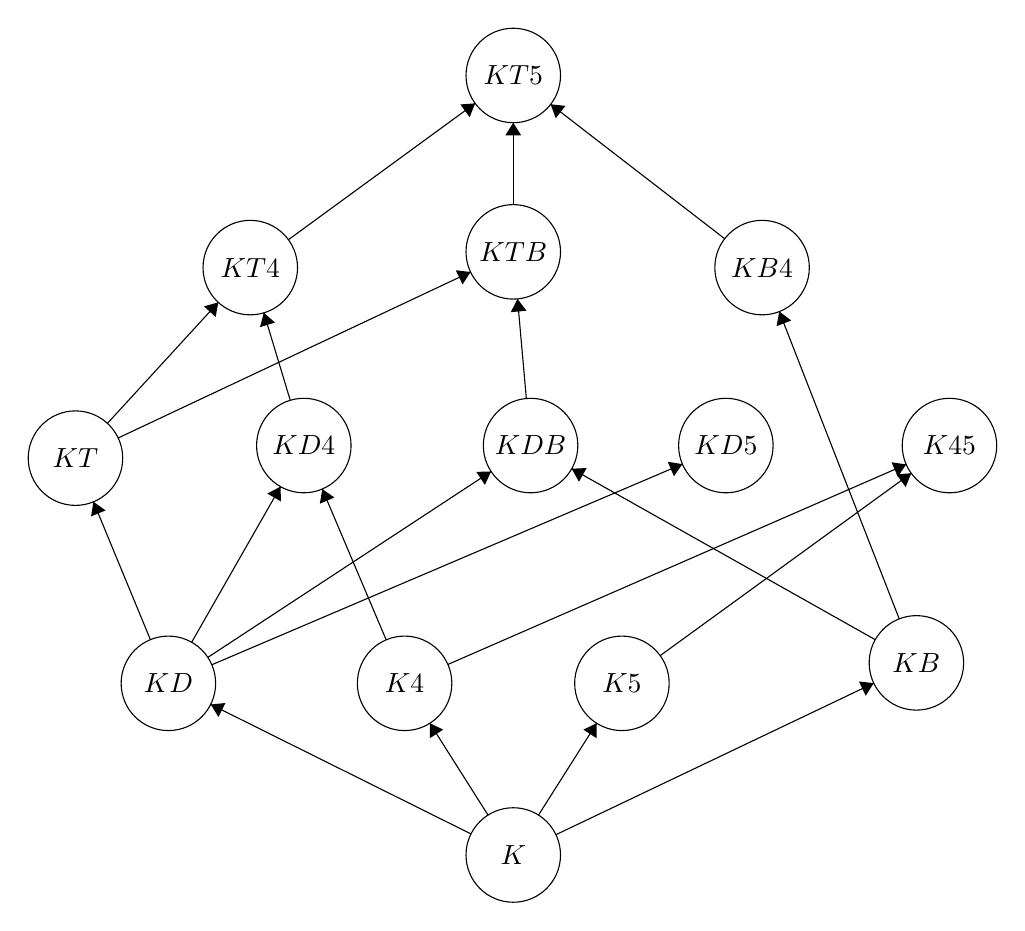
\begin{tikzpicture}[scale=0.2] \tikzstyle{every node}+=[inner sep=0pt] \draw [black] (39.9,-53.7) circle (3); \draw (39.9,-53.7) node {$K$}; \draw [black] (18,-42.8) circle (3); \draw (18,-42.8) node {$KD$}; \draw [black] (33,-42.8) circle (3); \draw (33,-42.8) node {$K4$}; \draw [black] (65.5,-41.5) circle (3); \draw (65.5,-41.5) node {$KB$}; \draw [black] (46.8,-42.8) circle (3); \draw (46.8,-42.8) node {$K5$}; \draw [black] (12.1,-28.5) circle (3); \draw (12.1,-28.5) node {$KT$}; \draw [black] (26.6,-27.7) circle (3); \draw (26.6,-27.7) node {$KD4$}; \draw [black] (53.4,-27.7) circle (3); \draw (53.4,-27.7) node {$KD5$}; \draw [black] (67.6,-27.7) circle (3); \draw (67.6,-27.7) node {$K45$}; \draw [black] (23.2,-16.4) circle (3); \draw (23.2,-16.4) node {$KT4$}; \draw [black] (39.9,-15.4) circle (3); \draw (39.9,-15.4) node {$KTB$}; \draw [black] (55.7,-16.4) circle (3); \draw (55.7,-16.4) node {$KB4$}; \draw [black] (39.9,-4.2) circle (3); \draw (39.9,-4.2) node {$KT5$}; \draw [black] (41,-27.7) circle (3); \draw (41,-27.7) node {$KDB$}; \draw [black] (37.21,-52.36) -- (20.69,-44.14); \fill [black] (20.69,-44.14) -- (21.18,-44.94) -- (21.62,-44.05); \draw [black] (38.3,-51.17) -- (34.6,-45.33); \fill [black] (34.6,-45.33) -- (34.61,-46.28) -- (35.45,-45.74); \draw [black] (42.61,-52.41) -- (62.79,-42.79); \fill [black] (62.79,-42.79) -- (61.85,-42.68) -- (62.28,-43.59); \draw [black] (41.5,-51.17) -- (45.2,-45.33); \fill [black] (45.2,-45.33) -- (44.35,-45.74) -- (45.19,-46.28); \draw [black] (16.86,-40.03) -- (13.24,-31.27); \fill [black] (13.24,-31.27) -- (13.09,-32.2) -- (14.01,-31.82); \draw [black] (14.13,-26.29) -- (21.17,-18.61); \fill [black] (21.17,-18.61) -- (20.26,-18.86) -- (21,-19.54); \draw [black] (25.74,-24.83) -- (24.06,-19.27); \fill [black] (24.06,-19.27) -- (23.82,-20.18) -- (24.77,-19.89); \draw [black] (31.83,-40.04) -- (27.77,-30.46); \fill [black] (27.77,-30.46) -- (27.62,-31.39) -- (28.54,-31); \draw [black] (19.48,-40.19) -- (25.12,-30.31); \fill [black] (25.12,-30.31) -- (24.28,-30.75) -- (25.15,-31.25); \draw [black] (20.76,-41.62) -- (50.64,-28.88); \fill [black] (50.64,-28.88) -- (49.71,-28.73) -- (50.1,-29.65); \draw [black] (35.75,-41.6) -- (64.85,-28.9); \fill [black] (64.85,-28.9) -- (63.92,-28.76) -- (64.32,-29.68); \draw [black] (49.23,-41.04) -- (65.17,-29.46); \fill [black] (65.17,-29.46) -- (64.23,-29.53) -- (64.82,-30.34); \draw [black] (64.41,-38.71) -- (56.79,-19.19); \fill [black] (56.79,-19.19) -- (56.62,-20.12) -- (57.55,-19.76); \draw [black] (62.89,-40.03) -- (43.61,-29.17); \fill [black] (43.61,-29.17) -- (44.07,-30) -- (44.56,-29.13); \draw [black] (20.51,-41.15) -- (38.49,-29.35); \fill [black] (38.49,-29.35) -- (37.55,-29.37) -- (38.1,-30.2); \draw [black] (14.81,-27.22) -- (37.19,-16.68); \fill [black] (37.19,-16.68) -- (36.25,-16.57) -- (36.68,-17.47); \draw [black] (40.73,-24.71) -- (40.17,-18.39); \fill [black] (40.17,-18.39) -- (39.74,-19.23) -- (40.74,-19.14); \draw [black] (25.62,-14.63) -- (37.48,-5.97); \fill [black] (37.48,-5.97) -- (36.54,-6.04) -- (37.13,-6.85); \draw [black] (39.9,-12.4) -- (39.9,-7.2); \fill [black] (39.9,-7.2) -- (39.4,-8) -- (40.4,-8); \draw [black] (53.33,-14.57) -- (42.27,-6.03); \fill [black] (42.27,-6.03) -- (42.6,-6.92) -- (43.21,-6.13); \end{tikzpicture} \end{center}

\textbf{\large{Somma diretta di Frame}}\textbf{}\\


S5 è determinata dalla classe dei frame d’ equivalenza (cioè frame
in cui la relazione di accessibilità è una relazione di equivalenza),
S5 = KT5 = KTB4 (riflessiva, simmetrica, transitiva)

S5 è determinata dalla classe dei frame universali (cioè frame in
cui la relazione di accessibilità è la relazione universale).

Mostriamo (almeno argomentiamo) la seconda affermazione.\\


Data una collezione di frame con insiemi di mondi a due a due disgiunti,
si dice somma diretta di questi frame il frame che ha come insieme
dei mondi l’unione dell’insieme dei mondi dei frame della collezione
e come relazione la unione delle relazioni dei frame della collezione.

$F=(S,R)$

$F1=(S1,R1)$, $F2=(S2,R2)$

$F=F1\oplus F2$ se e solo se $F=(S1\cup S2,\ R1\cup R2)$

Si dimostra che $\vera Fa$ se e solo se $\vera{F1}a$ e $\vera{F2}a$

Dato che una relazione di equivalenza forma una partizione sull'insieme
su cui è definita, e che in ogni classe di equivalenza è una relazione
universale, possiamo vedere una relazione di equivalenza come somma
di relazioni universali e il suo insieme come somma disgiunta di insiemi;
la somma diretta pertanto ci mostra quindi che S5 è determinata dai
frame universali.


\subsection{Tableau rivisitato per KT, KB}

Se una logica contiene l'assioma B devo aggiungere alle regole del
Tableau
\begin{itemize}
\item Regole di necessitazione\\
$\dfrac{\sigma\,\boa}{\sigma_{n}\, a}$ $\dfrac{\sigma\,\neg\dia}{\sigma_{n}\,\neg a}$
-- con $\sigma_{n}$ già presente nei nodi precedenti, oppure $\sigma_{n}$
\textbf{nodo corrente}
\end{itemize}
es. Si provi che la formula: $(\boa\implies a)$ è un teorema in KB

1: $\neg(\boa\implies a)$

1: $\boa$

1: $\neg a$

\textbf{1}: $a$ 

\begin{center}
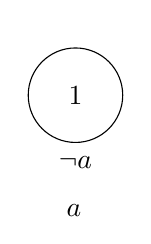
\begin{tikzpicture}[scale=0.2] 
\tikzstyle{every node}+=[inner sep=0pt] 
\draw [black] (26.8,-10.8) circle (3);
\draw (26.8,-10.8) node {1}; 

 
\draw (26.8,-6.6) node {$\boa$}; 

\draw (26.8,-15.1) node {$\neg{a}$};

\draw (26.7,-18.1) node {$a$}; 


\end{tikzpicture}
\end{center} 

Dove nell'ultimo passaggio ho usato proprio la regola appena introdotta,
avendo ottenuto $a$ e $\neg a$ nello stesso stato (mondo) deduco
che negare $a$ mi porta a un assurdo e quindi deve per forza essere
un teorema.\\
Se una logica contiene l'assioma T devo aggiungere alle regole del
Tableau
\begin{itemize}
\item Regole di necessitazione

\begin{itemize}
\item $\dfrac{\sigma\,\boa}{\sigma_{n}\, a}$ $\dfrac{\sigma\,\neg\dia}{\sigma_{n}\,\neg a}$
-- con $\sigma_{n}$ già presente nei nodi precedenti, oppure $\sigma_{n}$
\textbf{nodo prefisso del nodo corrente} (es 11 è prefisso di 111)
\end{itemize}
\end{itemize}
es. Si provi che la formula $(a\implies\boxx{\diamond a})$ è un teorema
in KT

1:$\neg(a\implies\boxx{\diamond a})$

1:$a$

1:$\neg(\boxx{\dia})$

1: $\diamond\boxx{\neg a}$

11: $\boxx{\neg a}$

\textbf{1: $\neg a$}

\begin{center} 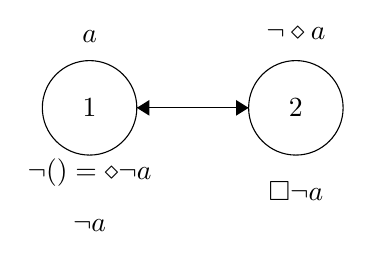
\begin{tikzpicture}[scale=0.2] \tikzstyle{every node}+=[inner sep=0pt] \draw [black] (26.7,-10.8) circle (3); \draw (26.7,-10.8) node {$1$};
\draw (26.7,-14.9) node {$\neg(\boxx{\dia})=\diamond\boxx{\neg a}$};
\draw (26.7,-18.3) node {$\neg a$}; \draw [black] (39.8,-10.8) circle (3); \draw (39.8,-10.8) node {$2$};
\draw (26.7,-6.3) node {$a$};
\draw (39.8,-6.1) node {$\neg\diamond a$};
\draw (39.8,-16.1) node {$\square\neg a$}; \draw [black] (29.7,-10.8) -- (36.8,-10.8); \fill [black] (36.8,-10.8) -- (36,-10.3) -- (36,-11.3); \draw [black] (36.8,-10.8) -- (29.7,-10.8); \fill [black] (29.7,-10.8) -- (30.5,-11.3) -- (30.5,-10.3); \end{tikzpicture} \end{center}


\end{document}
